\section{\review{Summary}}

This chapter examines the role of decapolar perturbations in the Large Hadron Collider (LHC) at
injection energy. First is addressed the previously observed discrepancy between measurements and
model regarding the third-order chromaticity. To investigate these issues, various measurements and
simulations were conducted. By introducing novel observables, such as the bare chromaticity and, for
the first time, chromatic amplitude detuning, a clearer understanding of these discrepancies was
achieved. Simulations indicate that the decay of the decapolar component in the main dipoles is a
major factor contributing to the discrepancies.

For the first time at injection energy, measurements and corrections of the decapolar Resonance
Driving Term (RDT) $f_{1004}$ were carried out. Further simulations and measurements explored how
sextupoles and octupoles interact to create decapolar-like fields. The findings revealed that
sextupoles, both alone and in combination with Landau octupoles, generate substantial decapolar RDTs
during machine operation that could benefit from corrections.

Applying combined corrections for third-order chromaticity, chromatic amplitude detuning, and the
RDT $f_{1004}$ led to a $3\%$ improvement in beam lifetime. Additionally, a broader impact of
decapolar RDTs on beam stability was investigated. Specifically, intentionally degrading the RDT
$f_{1004}$ resulted in a decrease in beam lifetime of about $10\%$. 
Furthermore, a significant improvement in the forced dynamic aperture during AC-Dipole excitation
was observed when corrections were applied. The earlier corrections for decapolar fields were
implemented alongside octupolar corrections for $Q''$. \Cref{fig:decapoles:losses_b4b5_corrs}
demonstrates the relative losses encountered when kicking at different amplitudes with the
AC-Dipole. This clearly shows that octupolar and decapolar corrections enhance the forced dynamic
aperture.

\begin{figure}[!htb]
    \centering
    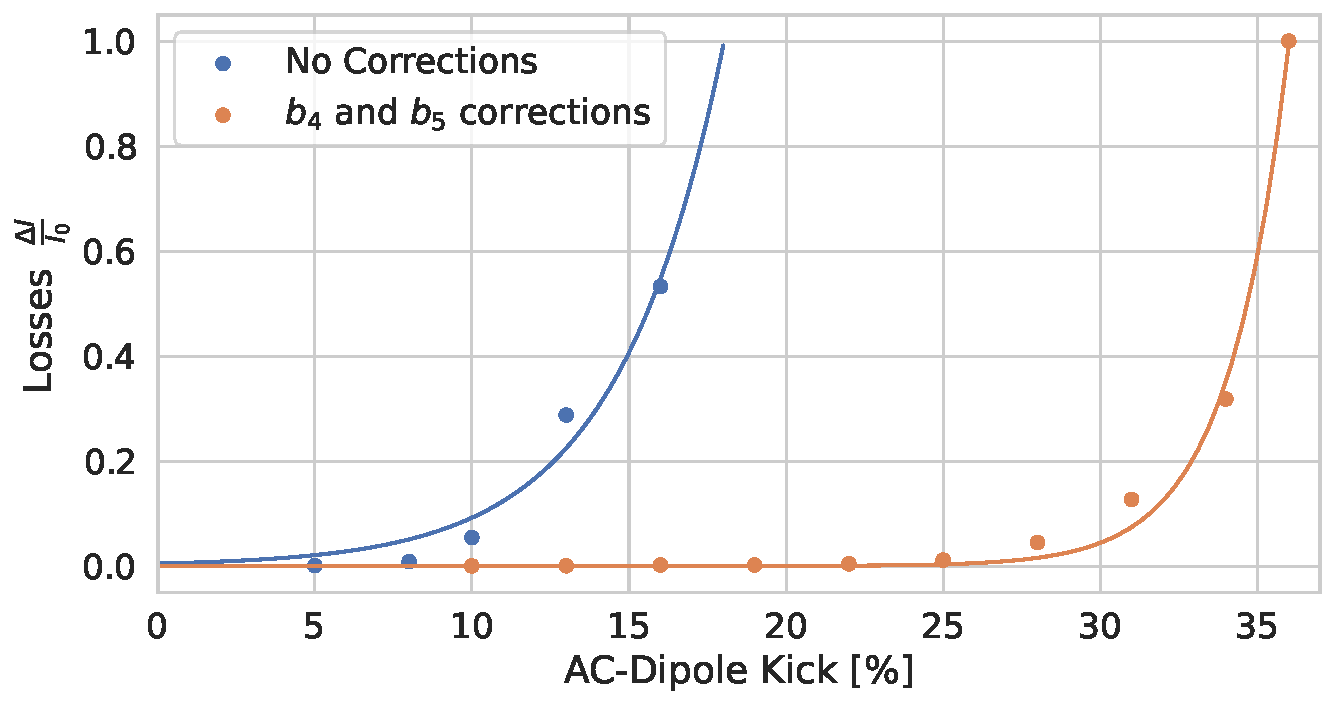
\includegraphics[width=0.8\textwidth]{./images/losses_with_without_b4b5corr.pdf}
    \caption{Relative losses experienced with AC-Dipole kick amplitude with and without corrections
    pertaining to $Q''$, $Q'''$, chromatic amplitude detuning, and RDT $f_{1004}$.}
    \label{fig:decapoles:losses_b4b5_corrs}
\end{figure}

This underscores the importance of these corrections for stable beam operation and suggests that
further advancements in correction methods could lead to even greater improvements. 